% ============================================================
% chapters/04-market.tex -- פרק 4: חקר שוק וכלים קיימים
% Content only. All design comes from template.cls.
% Figures: figures/ch4-market.tex (TikZ), figures/ch4-radar.pdf and
% figures/ch4-scatter.pdf (made by code/make_figures.py)
% ============================================================

\chapter{חקר שוק וכלים קיימים}
\label{ch:market}

בפרויקט מחקרי, ״השוק״ אינו קהל של לקוחות שקונים מוצר. השוק הוא הכלים, מאגרי הנתונים והשירותים שחוקרים משתמשים בהם היום כדי לענות על שאלות מסוג זה, והוא כולל גם את הדרך המסורתית: קריאה ידנית של המקורות. פרק זה בוחן את היקף התחום, סוקר את הכלים המרכזיים מבחינה טכנית, ומראה היכן המחקר המוצע משתלב ביניהם.

\section{היקף השוק בשלוש שכבות}
\label{sec:market-size}

את היקף השוק נהוג לתאר בשלוש שכבות (איור~\ref{fig:market-layers}): השוק הכולל (\en{TAM}), הפלח שהפתרון פונה אליו (\en{SAM}), והנתח המעשי שאפשר להגיע אליו בשנים הראשונות (\en{SOM}).

\begin{figure}[htbp]
  \centering
  % figures/ch4-market.tex -- three market layers TAM / SAM / SOM (chapter 4)
% Colors come from the template; fallbacks are defined here only if missing.
\providecolor{accent}{HTML}{8B2E2E}
\providecolor{accentlight}{HTML}{F4E9E1}
\begin{tikzpicture}[lab/.style={font=\small, align=center}]
  \fill[accentlight!60] (0,0) circle (36mm);
  \draw[accent, thick] (0,0) circle (36mm);
  \fill[accentlight] (0,-9mm) circle (25mm);
  \draw[accent, thick] (0,-9mm) circle (25mm);
  \fill[accent!25] (0,-17mm) circle (14mm);
  \draw[accent, thick] (0,-17mm) circle (14mm);
  \node[lab] at (0,26mm) {\textbf{\en{TAM}}\\ מדעי הרוח הדיגיטליים};
  \node[lab] at (0,7mm)  {\textbf{\en{SAM}}\\ חקר העת העתיקה\\ וימי הביניים המוקדמים};
  \node[lab] at (0,-17mm) {\textbf{\en{SOM}}\\ חוקרי המעבר\\ מרומא לימי הביניים};
\end{tikzpicture}

  \caption{שלוש שכבות השוק של המחקר המוצע}
  \label{fig:market-layers}
\end{figure}

\paragraph{השוק הכולל (\en{TAM}): מדעי הרוח הדיגיטליים.} דוחות מסחריים מגדירים תחום הכולל תוכנה, שירותים, ארכיונים וניתוח טקסט \cite{fds2026dh}. עם זאת, התקציר הציבורי של הדוח שנבדק אינו מספק נתוני בסיס ושיטת חישוב שמאפשרים לאמת אומדן כספי. לפיכך לא מוצג כאן גודל שוק בדולרים. בפרויקט פתוח שאינו מוכר מוצר, המדדים הרלוונטיים להיתכנות הם זמינות המקורות, היקף עבודת הקידוד ויכולת השימוש החוזר בתוצרים. אין לגזור מהם הכנסות או נתח שוק כספי.

\paragraph{הפלח הרלוונטי (\en{SAM}): כלים לחקר העת העתיקה וימי הביניים המוקדמים.} בתוך השוק הכולל, המחקר המוצע פונה לחוקרים, לסטודנטים ולמוסדות שעוסקים בהיסטוריה של העת העתיקה המאוחרת וימי הביניים המוקדמים, ובמיוחד בתחומים שבהם נדרש ניתוח טקסט ונתונים מובנים. לא נמצא מקור שמכמת את הפלח הזה בכסף, ולכן הוא מתואר לפי מי שפועל בו: הכלים שנסקרים בסעיף הבא משרתים בדיוק את הקהל הזה, וכולם מוצעים בגישה חופשית.

\paragraph{הנתח המעשי (\en{SOM}): קהילת המחקר על המעבר מרומא לימי הביניים.} בשנים הראשונות, הקהל המעשי של המחקר הוא חוקרים וקבוצות מחקר שעוסקים בשאלת נפילת רומא, בהתנצרות ובממלכות שקמו אחריה, ולצידם מורים ומרצים שמלמדים את התקופה. התוצרים – מאגר נתונים פתוח וקורפוס מתויג – יוצעו להם ללא תשלום, ולכן ״הנתח״ נמדד בשימוש ובציטוטים, ולא בהכנסות.

\section{סקירה טכנית של הכלים הקיימים}
\label{sec:market-tools}

הסקירה מתמקדת במה שכל כלי עושה בפועל, באיזה מידע הוא מחזיק, ומה חסר בו עבור שאלת המחקר.

\paragraph{\en{Seshat: Global History Databank}.} מאגר שנוסד ב־2011 ומקבץ באופן שיטתי את מה שידוע על הארגון החברתי והפוליטי של חברות אנושיות לאורך ההיסטוריה \cite{seshat_web}. האתר מפרסם נתוני שחזור של מחקרים, תמונות מצב תקופתיות וממשק גישה לנתונים. ב־21.11.2026 תמונת המצב המוצגת היא \en{Polaris-2026} \cite{seshat_web}; פרסום על המהדורה הקודמת מתאר את תהליך השחרור \cite{francois2025polaris}. המחקר ישמור עותק מתוארך של המהדורה שנבחרה, ולא יניח שמספר הישויות הכולל מבטיח כיסוי של שלושת המקרים. \textbf{החוזקה:} נתונים מובנים, מתועדים וזמינים לניתוח סטטיסטי, וזהו גם הבסיס של מאמר הדגל. \textbf{החולשה עבור המחקר:} יחידת הניתוח רחבה, והמאגר אינו מודד את אופן ההשתלבות של הכנסייה במוסדות המדינה.

\paragraph{\en{ORBIS}.} מודל ממוחשב של רשת התחבורה של הקיסרות הרומית, שפותח באוניברסיטת סטנפורד. המודל מחשב את הזמן והעלות של מסעות ביבשה, בנהרות ובים, ומשקף בעיקר את התנאים בסביבות שנת 200 לספירה \cite{scheidel2015orbis}. הוא כולל מאות אתרים ומשתרע על כעשרה מיליון קמ״ר, עם רשת דרכים של יותר מ־84 אלף ק״מ. \textbf{החוזקה:} כלי מצוין להבנת הקשר בין גיאוגרפיה, עלות ושליטה. \textbf{החולשה עבור המחקר:} הוא מתמקד בתקופה מוקדמת מתקופת המחקר ואינו עוסק בדת או במוסדות.

\paragraph{\en{Pleiades}.} מאגר גיאוגרפי (גזטיר) של מקומות עתיקים, שנבנה בידי קהילת חוקרים ומנוהל במכון לחקר העולם העתיק באוניברסיטת ניו יורק \cite{pleiades_web}. הוא מפרסם מקומות ומרחבים עתיקים ברישיון ייחוס פתוח; גודל המאגר אינו משמש כאן מדד לכיסוי התקופה. \textbf{החוזקה:} מזהים קבועים לכל מקום, שמאפשרים לקשר בין מאגרים שונים. \textbf{החולשה עבור המחקר:} הוא עוסק במקומות, לא באירועים או במוסדות.

\paragraph{\en{Perseus Digital Library} ו־\en{Scaife Viewer}.} ספרייה דיגיטלית חופשית לטקסטים יווניים ולטיניים, שמתארחת באוניברסיטת טאפטס \cite{perseus_scaife}. ממשק הקריאה \en{Scaife Viewer} מאפשר שימוש בקורפוסים של טקסטים יווניים ולטיניים; תיעוד המיזם וקודו פתוחים \cite{scaife_repository}. מספרי יצירות ומילים אינם מוצגים כאן, משום שהם תלויים בגרסת הקורפוס ואינם מעידים על זמינות המסמכים הדרושים למחקר. \textbf{החוזקה:} גישה פתוחה לטקסטים המקוריים ולתרגומים, בפורמט שהמחשב יכול לקרוא. \textbf{החולשה עבור המחקר:} הטקסטים אינם מתויגים לפי נושאים כמו יחסי כנסייה–מדינה, והאוסף מתמקד בספרות הקלאסית יותר מאשר במסמכי ממשל מאוחרים.

\paragraph{\en{dMGH} ו־\en{openMGH}.} המהדורה הדיגיטלית של \en{Monumenta Germaniae Historica}, הסדרה המרכזית של מקורות לתולדות ימי הביניים. כל כרכי המהדורה עברו דיגיטציה והם זמינים בגישה פתוחה, והכרכים הישנים ניתנים לחיפוש בטקסט מלא; כרכים חדשים מצטרפים אחרי תקופת המתנה של שנתיים \cite{mgh_dmgh}. במסגרת \en{openMGH} מוצעים הטקסטים גם כקובצי \en{TEI-XML} ברישיון פתוח \cite{mgh_openmgh}. \textbf{החוזקה:} זהו מקור מרכזי לחקיקה, להחלטות מועצות ולכרוניקות של הממלכה הפרנקית – בדיוק סוג הטקסטים שממנו נגזרים מדדי ההשתלבות המוצעים. \textbf{החולשה עבור המחקר:} אין בו ניתוח, סיווג או נתונים מובנים; את כל זה צריך לבנות.

\paragraph{\en{Ithaca}.} דוגמה לכלי \en{AI} ייעודי לטקסטים עתיקים: רשת נוירונים שמשחזרת כתובות יווניות פגומות, מזהה את מקומן ומתארכת אותן \cite{assael2022ithaca}. \textbf{החוזקה:} הוכחה לכך שמודלים יכולים לעבוד עם שפות עתיקות, במיוחד בשיתוף עם היסטוריונים. \textbf{החולשה עבור המחקר:} הכלי מיועד לכתובות ולא לסיווג תוכן של טקסטים ספרותיים ומשפטיים.

\paragraph{קריאה ידנית של המקורות.} זהו ״המתחרה האמיתי״ של כל מחקר כמותי: היסטוריון שקורא את המקורות, מסכם אותם ומסיק מסקנות. \textbf{החוזקה:} עומק, הבנת הקשר ויכולת לזהות ניואנסים. \textbf{החולשה:} קריאה וקידוד של אלפי טקסטים משלוש מדינות דורשים זמן רב וספר קידוד מפורש כדי לאפשר בדיקה ושחזור.

\section{טבלת השוואה רב־פרמטרית}
\label{sec:market-table}

טבלה~\ref{tab:market-compare} מרכזת את הכלים לפי הפרמטרים שחשובים למחקר המוצע, לצד מאמר הדגל והמחקר המוצע.

\begin{table}[htbp]
  \centering
  \caption{השוואה בין הכלים הקיימים, מאמר הדגל והמחקר המוצע}
  \label{tab:market-compare}
  \small
  \begin{tabular}{p{26mm}p{24mm}p{24mm}p{22mm}p{16mm}p{24mm}}
    \toprule
    \textbf{כלי} & \textbf{סוג המידע} & \textbf{כיסוי התקופה \LR{312--843}} & \textbf{כנסייה ומדינה} & \textbf{גישה} & \textbf{מה חסר לנו} \\
    \midrule
    \en{Seshat} & נתונים מובנים על ישויות מדיניות & חלקי, ברזולוציה גסה & קטגוריית דת כללית & פתוחה & מדדי השתלבות \\
    \en{ORBIS} & רשת תחבורה, זמן ועלות & סביב שנת 200 & לא & פתוחה & כמעט הכול \\
    \en{Pleiades} & מקומות ושמות & רחב & לא & פתוחה & אירועים ומוסדות \\
    \en{Perseus / Scaife} & טקסטים מקוריים ותרגומים & חלקי & בתוך הטקסטים & פתוחה & תיוג נושאי \\
    \en{dMGH / openMGH} & מהדורות מקורות & רלוונטי לפרנקים & בתוך הטקסטים & פתוחה & ניתוח ונתונים מובנים \\
    \en{Ithaca} & מודל \en{AI} לכתובות & לא ממוקד & לא & קוד פתוח & סיווג תוכן \\
    קריאה ידנית & פרשנות של חוקר & תלוי בחוקר & כן, איכותני & – & היקף ועקביות \\
    \midrule
    מאמר הדגל \cite{turchin2022disentangling} & מודל סטטיסטי על \en{Seshat} & חלקי & לא ממוקד & נתונים פתוחים & מיקוד ורזולוציה \\
    \textbf{המחקר המוצע} & \textbf{מאגר + קורפוס מתויג} & \textbf{יעד: 3 מדינות} & \textbf{כן, כמותי} & \textbf{פתוחה} & – \\
    \bottomrule
  \end{tabular}
\end{table}

\section{שני גרפים שמספרים את הסיפור}
\label{sec:market-graphs}

שני הגרפים הבאים מציגים את אותה השוואה בצורה חזותית. הציונים (1 עד 5) הם \textbf{הערכה של צוות המחקר}, המבוססת על הסקירה שבסעיף~\ref{sec:market-tools}; הם נועדו להמחיש את ההבדלים בין הכלים, ואינם מדידה.

תרשים הרדאר (איור~\ref{fig:market-radar}) מראה את הפרופיל של כל כלי על שישה צירים. כל אחד מהכלים הקיימים חזק בצירים מסוימים: \en{Seshat} בנתונים מובנים, \en{Perseus} ו־\en{dMGH} בגישה פתוחה לטקסטים, \en{Pleiades} בקריאה במחשב. אף אחד מהם אינו חזק בו־זמנית במידע על כנסייה ומדינה ובניתוח טקסט, ושם בדיוק נמצא המחקר המוצע.

\begin{figure}[htbp]
  \centering
  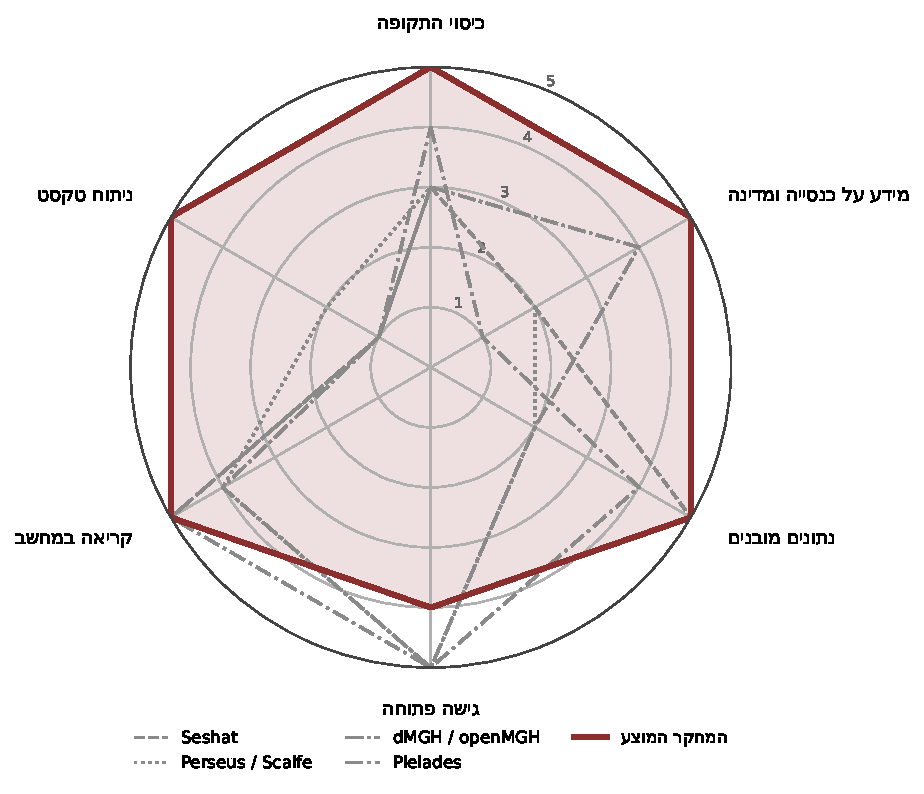
\includegraphics[width=0.78\textwidth]{figures/ch4-radar.pdf}
  \caption{פרופיל הכלים על שישה צירים (הערכת הצוות, להמחשה)}
  \label{fig:market-radar}
\end{figure}

גרף הפיזור (איור~\ref{fig:market-scatter}) מציב כל כלי לפי שני ממדים: כמה משאלת המחקר הוא עונה, וכמה מאמץ נדרש כדי להשתמש בו לצורך זה. הכלים הקיימים מתחלקים לשתי קבוצות: כלים שקל להשתמש בהם אבל הם עונים על חלק קטן מהשאלה (\en{Pleiades}, \en{ORBIS}, \en{Seshat}), וכלים שעונים על יותר אבל דורשים מאמץ רב (\en{dMGH}, קריאה ידנית). המחקר המוצע מכוון לפינה הימנית התחתונה: לענות על רוב השאלה, במאמץ סביר – כי העבודה הכבדה של קריאה וסיווג נעשית פעם אחת, ותוצריה פתוחים לכולם.

\begin{figure}[htbp]
  \centering
  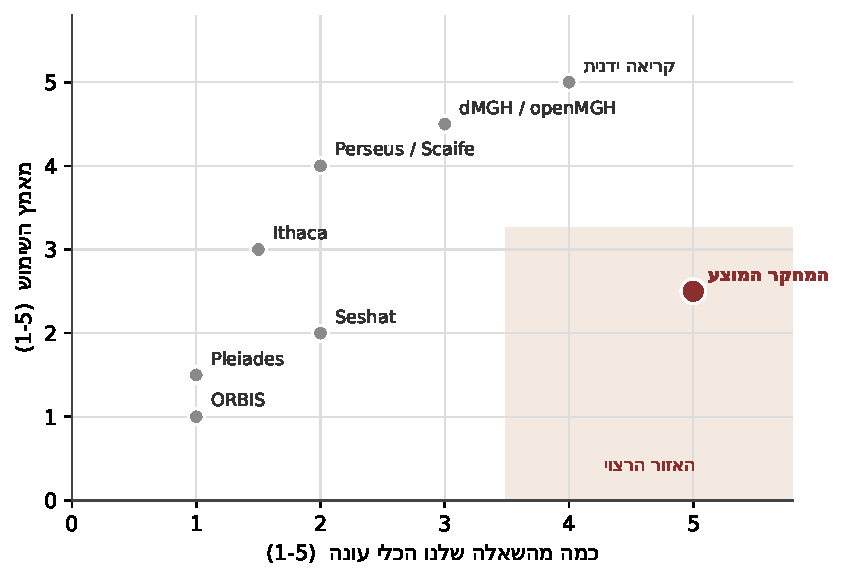
\includegraphics[width=0.78\textwidth]{figures/ch4-scatter.pdf}
  \caption{כמה מהשאלה כל כלי עונה, מול מאמץ השימוש (הערכת הצוות, להמחשה)}
  \label{fig:market-scatter}
\end{figure}

\section{מסקנות: לא מתחרים, אלא שכבה חדשה}
\label{sec:market-conclusion}

הסקירה מובילה לשלוש מסקנות. ראשית, \textbf{הכלים שנסקרו אינם מספקים לבדם תשובה לשאלת המחקר}, אבל זה לא משום שאיש לא עבד בתחום: יש כלים מצוינים, וכל אחד מהם פותר חלק אחר של הבעיה. שנית, \textbf{המחקר המוצע לא מתחרה בכלים האלה, אלא נבנה עליהם}: הטקסטים יגיעו מ־\en{Perseus} ומ־\en{dMGH}, משתני הפיקוח יגיעו בחלקם מ־\en{Seshat}, והמקומות יקושרו למזהים של \en{Pleiades}. שלישית, \textbf{הכלים שנסקרו מציעים גישה פתוחה למשאבים מרכזיים}, ולכן גם התוצרים המוצעים יהיו פתוחים. העלות האמיתית של המחקר אינה רישיונות, אלא זמן של חוקרים ועלות של טוקנים במודלי שפה – ואת שתיהן נבחן בפרקים~\ref{ch:alternatives} ו־\ref{ch:workplan}.


\section{בדיקת היתכנות של מקורות הנתונים}
\label{sec:market-access}

גישה לאתר אינה מבטיחה שמותר להוריד ולפרסם כל פריט בו. לפני איסוף הקורפוס תיבנה רשימת מהדורות: מחבר, תאריך, שפה, מדינה, סוג מקור, כתובת קבועה ותנאי שימוש. ב־\en{openMGH} קובצי המהדורות מוצעים כ־\en{TEI-XML} ברישיון \en{CC BY 4.0} \cite{mgh_openmgh}; ב־\en{Pleiades} התוכן מופץ ברישיון ייחוס \cite{pleiades_web}. רישיון התוכנה של \en{Scaife} אינו מחליף בדיקה של רישיון המהדורה או התרגום. כשאין היתר להפיץ טקסט, יפורסמו רק מזהים, תיוגים ומראי מקום, בהתאם לתנאי המקור.

לכל אחת משלוש המדינות תיבחן בנפרד זמינותם של חוקים, מכתבים, החלטות מועצות וכרוניקות. יעד של 2,000 קטעים אינו הוכחה שהחלוקה ביניהן מאוזנת. בחודש הראשון תיבדק זמינות של לפחות 50 קטעים מועמדים מכל מדינה ולפחות שני סוגי מקורות בכל מקרה. זו בדיקת היתכנות עתידית, ולא תוצאה שכבר התקבלה. אם מקרה אינו עומד בסף, יש לאתר מאגר נוסף או להציג לאישור שינוי היקף; אין להשלים טקסטים חסרים באמצעות מודל שפה.

הציונים בגרפים משקפים הערכה מקדימה. הציון הגבוה של המחקר המוצע מתאר יעד תכן, ולא ביצועים שנמדדו. בשלב הביצוע ייבדקו הכיסוי בפועל, שיעור הרשומות בעלות מקור ותאריך, שיעור שגיאות הסיווג וזמן השימוש בתוצר. כך יהיה אפשר להחליף הערכה במדידה בלי לשנות בדיעבד את הגדרת ההצלחה.
